\documentclass[final]{beamer}

% ====================
% Packages
% ====================

\usepackage[T1]{fontenc}
\usepackage{lmodern}
\usepackage[size=custom,width=121.92,height=91.44,scale=1.05]{beamerposter}
\usetheme{poster}
\usecolortheme{labsix}
\usepackage{graphicx}
\usepackage{booktabs}
\usepackage{tikz}
\setbeamertemplate{caption}{%
  \raggedright
  \insertcaption\par
}

\usepackage{pgfplots}
\usepackage{array} % for spacing tables out \extrarowheight
%\pgfplotsset{compat=1.15}

% ====================
% Lengths
% ====================

% If you have N columns, choose \sepwidth and \colwidth such that
% (N+1)*\sepwidth + N*\colwidth = \paperwidth
\newlength{\sepwidth}
\newlength{\colwidth}
\setlength{\sepwidth}{0.04375\paperwidth}
\setlength{\colwidth}{0.275\paperwidth}

% Spacing / Formatting
\newcommand{\separatorcolumn}{\begin{column}{\sepwidth}\end{column}}
\newcommand{\itembox}[1]{\item {\makebox[10cm]{#1 \hfill}}}

% Standard Probability
\DeclareMathOperator{\E}{\mathbb{E}}
\newcommand{\PP}{\mathbb{P}}
\newcommand{\RR}{\mathbb{R}}

% Data-Consistent Inversion Framework

\DeclareMathOperator*{\param}{\lambda}
\newcommand{\pspace}{\Lambda}
\newcommand{\pmeas}{\mu_{\pspace}}
\newcommand{\pborel}{\mathcal{B}_{\pspace}}

\DeclareMathOperator*{\initialP}{\PP_{in}}
\DeclareMathOperator*{\initial}{\pi_{in}}
\DeclareMathOperator*{\updatedP}{\PP_{up}}
\DeclareMathOperator*{\updated}{\pi_{up}}

\DeclareMathOperator*{\noise}{\xi}
\DeclareMathOperator*{\nspace}{\Xi}

\newcommand{\obs}{\boldsymbol{o}}
\newcommand{\data}{\boldsymbol{d}}
\newcommand{\dspace}{\mathcal{D}}
\newcommand{\dmeas}{\mu_{\dspace}}
\newcommand{\dborel}{\mathcal{B}_{\dspace}}

\DeclareMathOperator*{\lam}{\left ( \param \right ) }
\DeclareMathOperator*{\qoi}{Q \lam }
\DeclareMathOperator*{\qlam}{\left ( \qoi \right ) }

\DeclareMathOperator*{\observedP}{\PP_{obs}}
\DeclareMathOperator*{\observed}{\pi_{obs}}
\DeclareMathOperator*{\predictedP}{\PP_{pre}}
\DeclareMathOperator*{\predicted}{\pi_{pre}}

\DeclareMathOperator*{\dciP}{\updatedP = \initialP \frac{\observedP}{\predictedP}}
\DeclareMathOperator*{\dciD}{\updated = \initial \frac{\observed}{\predicted}}
\DeclareMathOperator*{\dci}{\updated\lam = \initial\lam \frac{\observed\qlam}{\predicted\qlam}}

% Bayesian Framework
\DeclareMathOperator*{\hyperparam}{\alpha,\beta}
\newcommand{\hyperspace}{\Omega}

\DeclareMathOperator*{\hyper}{\left ( \hyperparam \right ) }
\DeclareMathOperator*{\lamGiveq}{\left ( \param \mid \data \right ) }
\DeclareMathOperator*{\qGivelam}{\left ( \data \mid \param \right ) }
\DeclareMathOperator*{\qGivelamH}{\left ( \data \mid \param,\hyperparam \right ) }
\DeclareMathOperator*{\lamGiveH}{\left ( \param \mid \hyperparam \right ) }

\DeclareMathOperator*{\prior}{\pi_{prior}}
\DeclareMathOperator*{\posterior}{\pi_{post}}
\DeclareMathOperator*{\likelihood}{\pi_{L}}

\DeclareMathOperator*{\bayes}{\posterior\lamGiveq \propto \prior\lam \likelihood\qGivelam}
\DeclareMathOperator*{\Hbayes}{\posterior\lamGiveq \propto \int_\hyperspace \prior\hyper \prior\lamGiveH \likelihood\qGivelamH\,d\hyperspace}



% ====================
% Title
% ====================

\title{Using Push-Forward and Pullback Measures for Parameter Identification and Distribution Estimation}

\author{\color{black} Tian Yu Yen and Michael Pilosov}
%\institute[shortinst]{\color{black} under the direction of Dr. Troy Butler at the University of Colorado: Denver}
\institute[shortinst]{\color{black} University of Colorado: Denver}

% ====================
% Body
% ====================

\begin{document}

\begin{frame}[t]
\center\heading{THIS IS A BIG-ASS HEADING}
\begin{columns}[t]
\separatorcolumn

\begin{column}{\colwidth}

  \begin{block}{Introduction}
\centering
        \heading{Motivation} 
            {\large How do we update initial descriptions of uncertainty using model predictions and data?}

        %\heading{Background}
             %{\large \emph{Data Consistent Inversion} is a Measure-Theoretic Framework for the solution of stochastic inverse problems. }
             {\large \textbf{Data-Consistent Inversion} is a novel framework that uses push-forward and pull-back measures to ensure solutions are consistent with the observed distribution of data.}

        \heading{Question} 
             {\large \emph{How do we cast a \textbf{Parameter Identification} problem in the context of Data-Consistent Inversion?} }

\end{block}

\begin{block}{Framework}

\centering
\vspace{1cm}
    \heading{Updating with Observations and Predictions}
    \begin{equation*}
            \dciP \quad \vline \quad \dci
    \end{equation*}
    %\begin{equation*}
    %        \dci
    %\end{equation*}

\end{block}



\end{column}

\separatorcolumn

\begin{column}{\colwidth}
  \begin{block}{Intro to Data Consistent Inversion}
\centering
        \heading{Solving Stochastic Inverse Problems} 
            %{\large How do we update initial descriptions of uncertainty using model predictions and data?}

        %\heading{Background}
             %{\large \emph{Data Consistent Inversion} is a Measure-Theoretic Framework for the solution of stochastic inverse problems. }
             {\large \textbf{Data-Consistent Inversion} is a novel framework that uses push-forward and pull-back measures to ensure solutions are consistent with the observed distribution of data.}

        %\heading{Question} 
         %    {\large \emph{How do we cast a \textbf{Parameter Identification} problem in the context of Data-Consistent Inversion?} }
\vspace{0.5cm}
\heading{The Data Consistent Approach}
\[ \scalebox{1.5}{$\dci$} \]


\end{block}


\begin{block}{Which Stochastic Inverse Problem?}
\centering

% \vspace{1cm}
% \heading{Quantity of Interest Map}
%     \emph{\large A Functional Relating \textbf{Predictions} and \textbf{Data}}
%     \large
%     \begin{itemize}
%        \itembox{Ideal} $Q \left (\param, \noise \right ) = F \left ( \obs(\param), \data(\noise) \right )$
%        \itembox{Theoretical} $Q \left ( \pspace, \nspace \right ) =: \dspace_\mathcal{T} \subset \RR$
%        \itembox{Practical} $Q \left (\param \right ) = F \left ( \obs(\param), \data^\dagger \right )$
%        \itembox{Computable} $Q \left ( \pspace \right ) =: \dspace_\mathcal{C} \subset \dspace_\mathcal{T}$
%     \end{itemize}
    \begin{figure}
        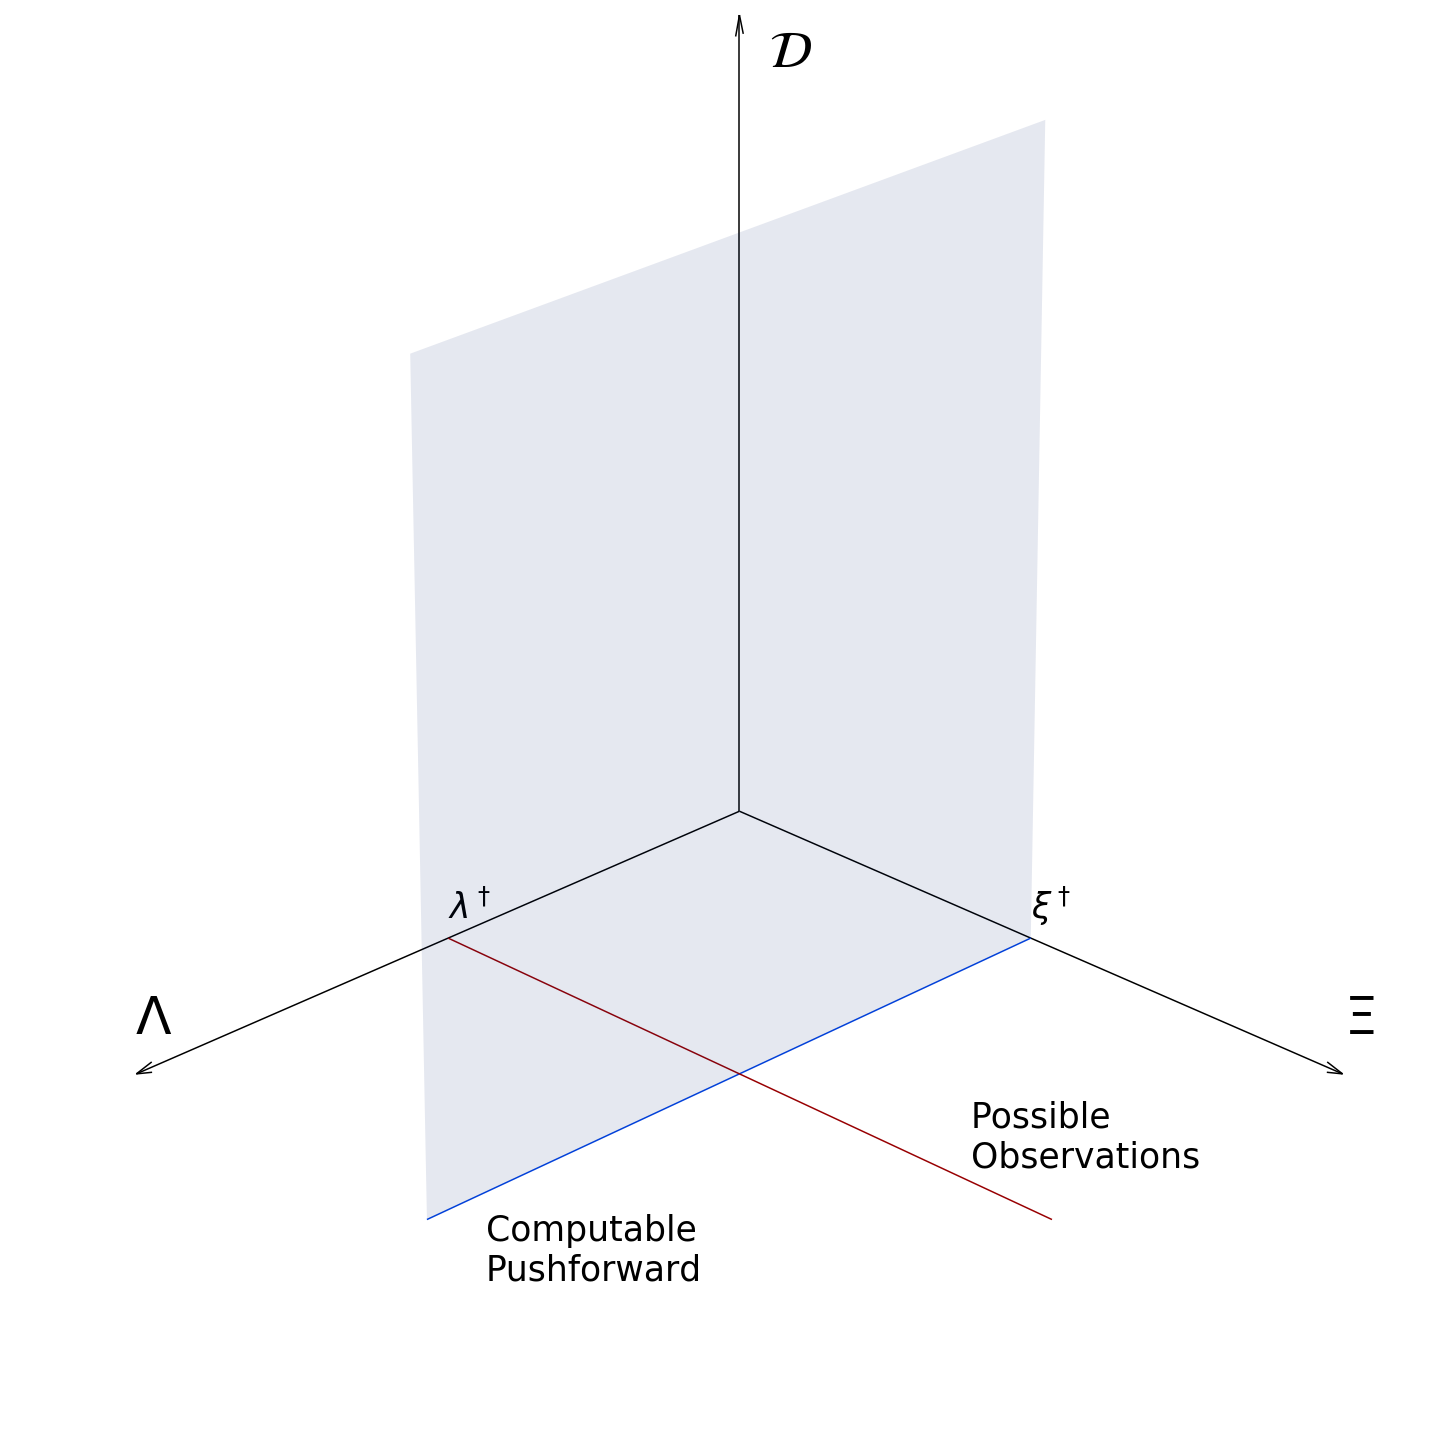
\includegraphics[height=23cm]{figures/diagram}
    \caption{\large \emph Do you want to solve for a single parameter value or for a parameter distribution?}
    \end{figure}


% \vspace{1cm}
% \heading{Observed Distribution}
% {\large \emph Given a functional, what measure do we invert?}

% \Large
%     $Q(\param^\dagger, \noise) \sim \observed$ when we allow $\noise$ to vary over $\nspace$
%     \begin{table}
%       \centering
%       {\setlength{\tabcolsep}{0.25em}
%       \begin{tabular}{c <{\hspace{1pc}} c >{\hspace{1pc}} c}
%         %\toprule
%         %\large
%         \textbf{$F(\obs(\param), \data^\dagger)$} & \textbf{$\noise$} & {$\observed$} \\
%         \midrule
%         $\frac{1}{\sigma\sqrt{D}} \large\sum \left( \obs_i\lam - \data_i^\dagger \right)$ & $ \noise \sim L^2$ & $N(0,1) $ \\[1.5ex]
%         $\frac{1}{\sigma^2} \large\sum \left ( \obs_i\lam - \data_i^\dagger \right)^2$ & $ \noise \sim N(0,\sigma^2) $ & $\chi^2 (D)$ \\[1.5ex]
%         $\frac{1}{\sigma^2 D} \large\sum \left ( \obs_i\lam - \data_i^\dagger \right)^2$ & $ \noise \sim N(0,\sigma^2) $ & $ \Gamma \left ( D/2, D/2) \right ) $ \\
%         \normalsize\vdots & \normalsize\vdots & \normalsize\vdots \\
%         %\bottomrule
%       \end{tabular}
%       }
%       \caption{Choices of $F$ and associated $\observed$ for stochastic inverse problem with $\data^\dagger = \obs_i(\param^\dagger) + \xi_i^\dagger$
% }
%     \end{table}

%
\end{block}

  \begin{block}{Notation}
\centering
\large
    \begin{itemize}
        \itembox{$ \PP, \; \pi $} Probability Measure, Density
        %\itembox{$ \pi $} Density (Radon-Nikodym)
        \itembox{$\pspace \subset \RR^P$} Parameter Space
        \itembox{$\obs: \pspace \to \mathcal{O} \subset \RR^D$} Observables
        \itembox{$\nspace \subset \RR^D$} Noise Space
        \itembox{$\param^\dagger\in\pspace$} True Parameter
        \itembox{$\data(\noise) \subset \RR^D$} Possible Data, $d_i(\noise) = \obs_i(\param^\dagger) + \xi_i$
        \itembox{$\noise^\dagger\in\nspace$} Noise in Measurements
        \itembox{$ \sigma^2 $} Variance of Noise
        \itembox{$\data^\dagger\in\RR^D$} Observed Data, $\data^\dagger = \data(\noise^\dagger)$
        \itembox{$ \initialP, \; \initial $} Initial
        \itembox{$ \observedP, \; \observed $} Observed
        \itembox{$ \predictedP, \; \predicted $} Predicted (\textbf{push-forward})
        \itembox{$ \updatedP, \; \updated $} Updated (\textbf{pull-back})
    \end{itemize}

\end{block}
%   \vspace{-0.5cm}
  \begin{block}{References \& Attribution}
    \centering
    \textbf{Advisor: Dr. Troy Butler}
    \begin{figure}
        
\includegraphics[width=3cm]{figures/ref-theory}
        
\includegraphics[width=3cm]{figures/ref-stability}
        
\includegraphics[width=3cm]{figures/ref-bet}
        
\includegraphics[width=3cm]{figures/ref-cb}
        
\includegraphics[width=3cm]{figures/ref-website}
    \caption{\centering Left to Right: Theory, Stability, BET, ConsistentBayes, Personal Website. \newline Funding provided by NSF DMS-1818941.}
    \end{figure}

    %\nocite{*}
    %\footnotesize{\bibliographystyle{plain}\bibliography{poster}}
\end{block}


  
\end{column}

\separatorcolumn

\begin{column}{\colwidth}

  \begin{block}{Parameter Identification}
\centering
        \heading{Goal: Obtain the Best Value of $\lambda$} 
%             {\large \textbf{Bayesian Context:} Regular Bayes model uses assumed likelihood function of data given $\lambda$.}
            
%             {\large \textbf{Data Consistent Context:} Uses data to construct a predicted distribution of the average residuals given $\lambda$.}
        \begin{itemize}
            \itembox{\bf \large Bayesian Context:} Model uses assumed likelihood function of data given $\lambda$.
            \itembox{\bf \large Data Consistent:} Construct predicted distribution of residuals given $\lambda$.
        \end{itemize}            
            %{\large How do we update initial descriptions of uncertainty using model predictions and data?}

        %\heading{Background}
             %{\large \emph{Data Consistent Inversion} is a Measure-Theoretic Framework for the solution of stochastic inverse problems. }
             %{\large \textbf{Data-Consistent Inversion} is a novel framework that uses push-forward and pull-back measures to ensure solutions are consistent with the observed distribution of data.}

        %\heading{Question} 
          %   {\large \emph{How do we cast a \textbf{Parameter Identification} problem in the context of Data-Consistent Inversion?} }

\end{block}

% \vspace{-0.5cm}

\begin{block}{Example}
\centering
    Consider an exponential decay problem with uncertain decay rate:
   \begin{equation*}
       u(t) = u_0\exp(-\lambda t), \; u_0 = 0.5 ,\; t\in[0,3]
   \end{equation*}
\vspace{-0.5cm}
    \begin{figure}
        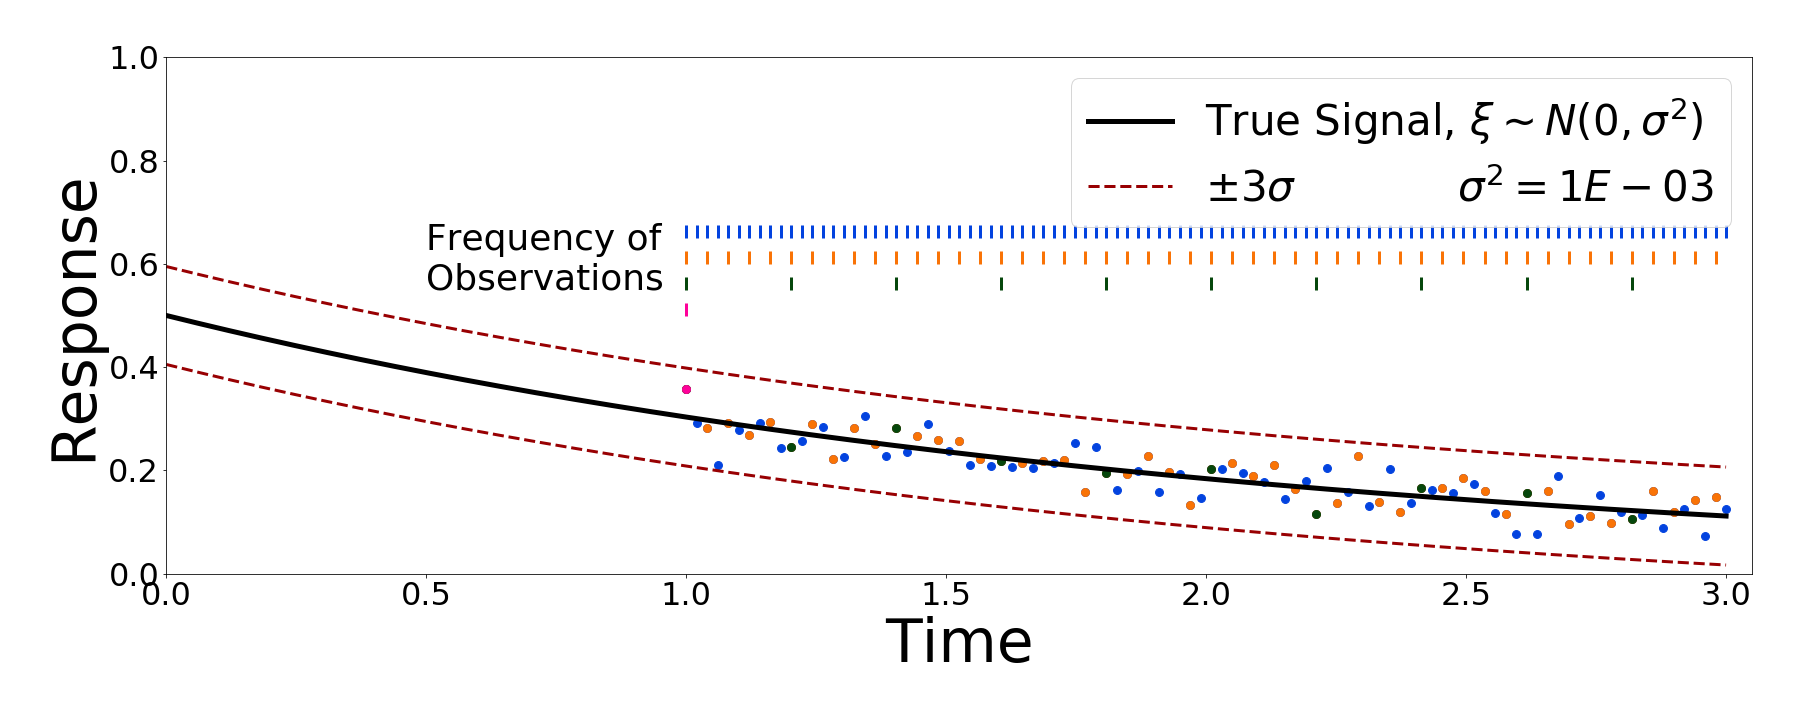
\includegraphics[width=26cm]{figures/exponential_decay_response_sigma-10E-4}
    \end{figure}

%\end{block}

% \vspace{-0.5cm}

%\begin{block}{Convergence}
\centering
\heading{Convergence of Data Consistent Inversion}
{\emph How do solutions change with more data?}
% \vspace{-0.5cm}
    \begin{figure}
        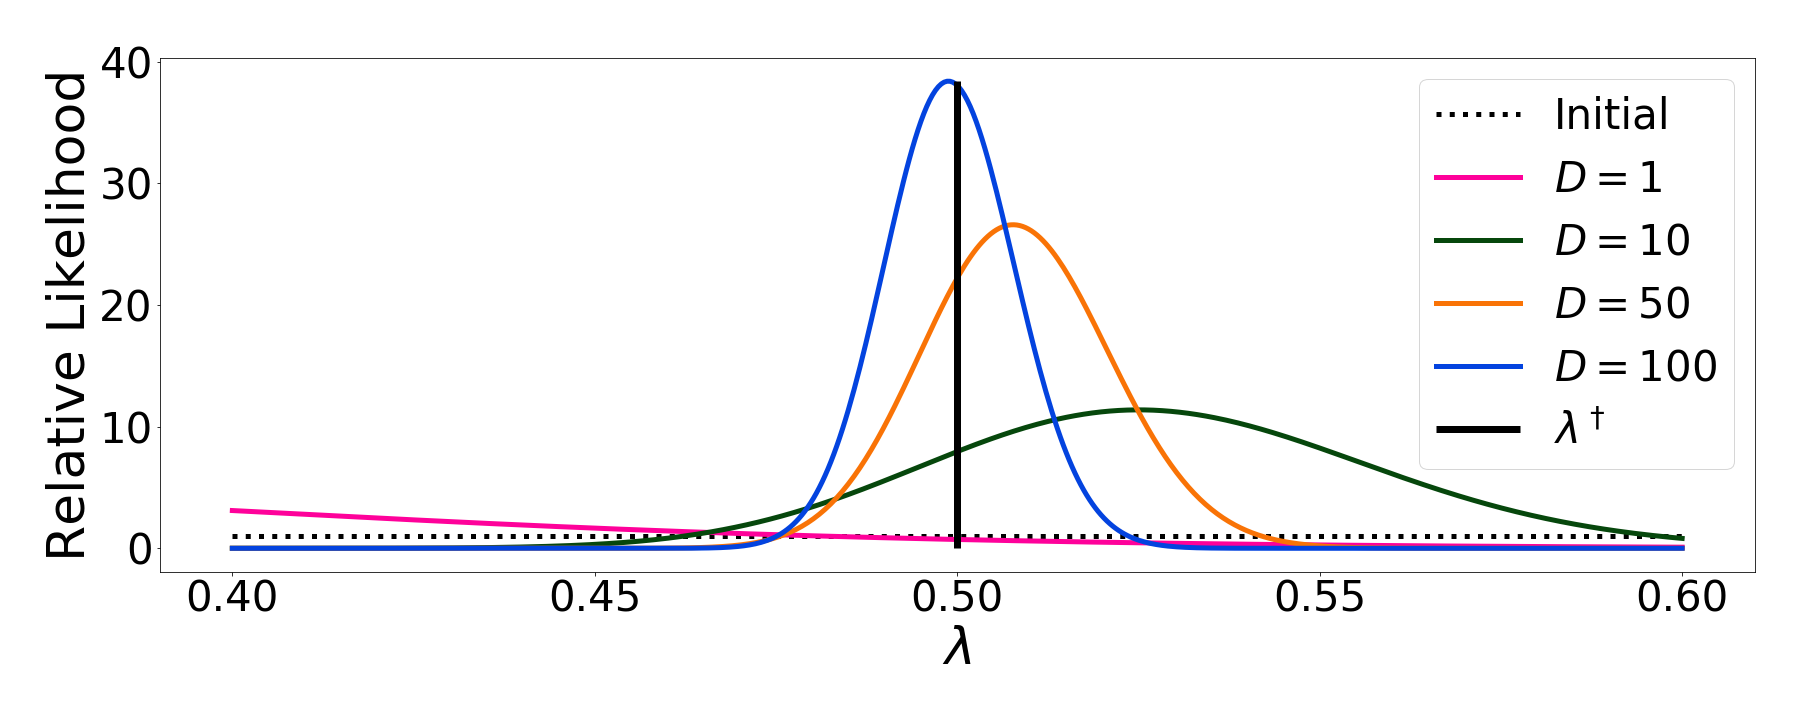
\includegraphics[width=26cm]{figures/updated_convergence_sigma-10E-4}
        \vspace{-0.5cm}
        \caption{ $\param^\dagger$ and $\updated$ for $D=1, 10, 50, 100$ for $N=1000$}
    \end{figure}

%\end{block}

% \vspace{-0.5cm}

%\begin{block}{Stability}
\heading{Comparison to Regular Bayes}
{\emph How do solutions on conditionals of $\nspace$ compare?}
% \vspace{-0.5cm}
    \begin{figure}
        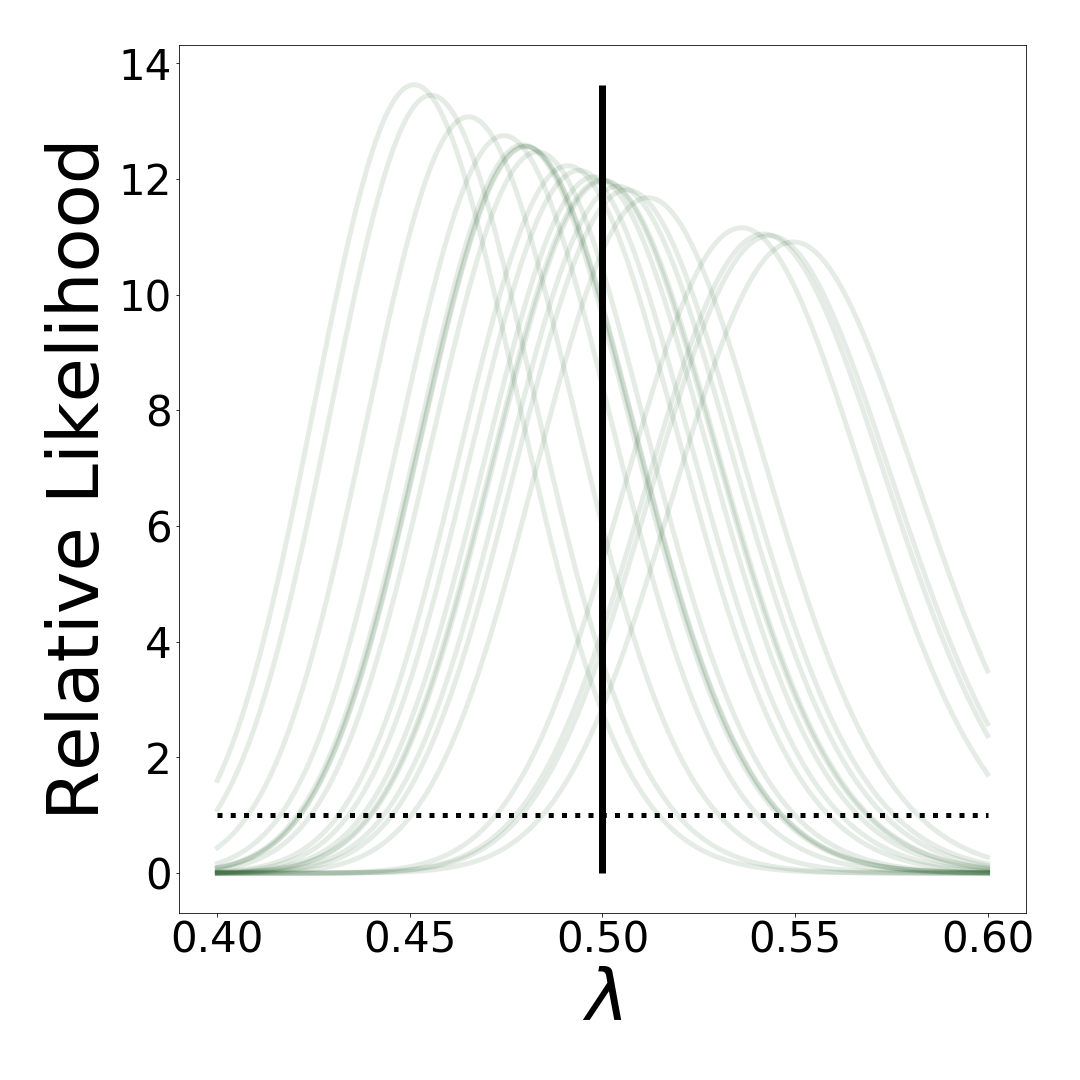
\includegraphics[width=13cm]{figures/updated_stability_D10_sigma-10E-4}
        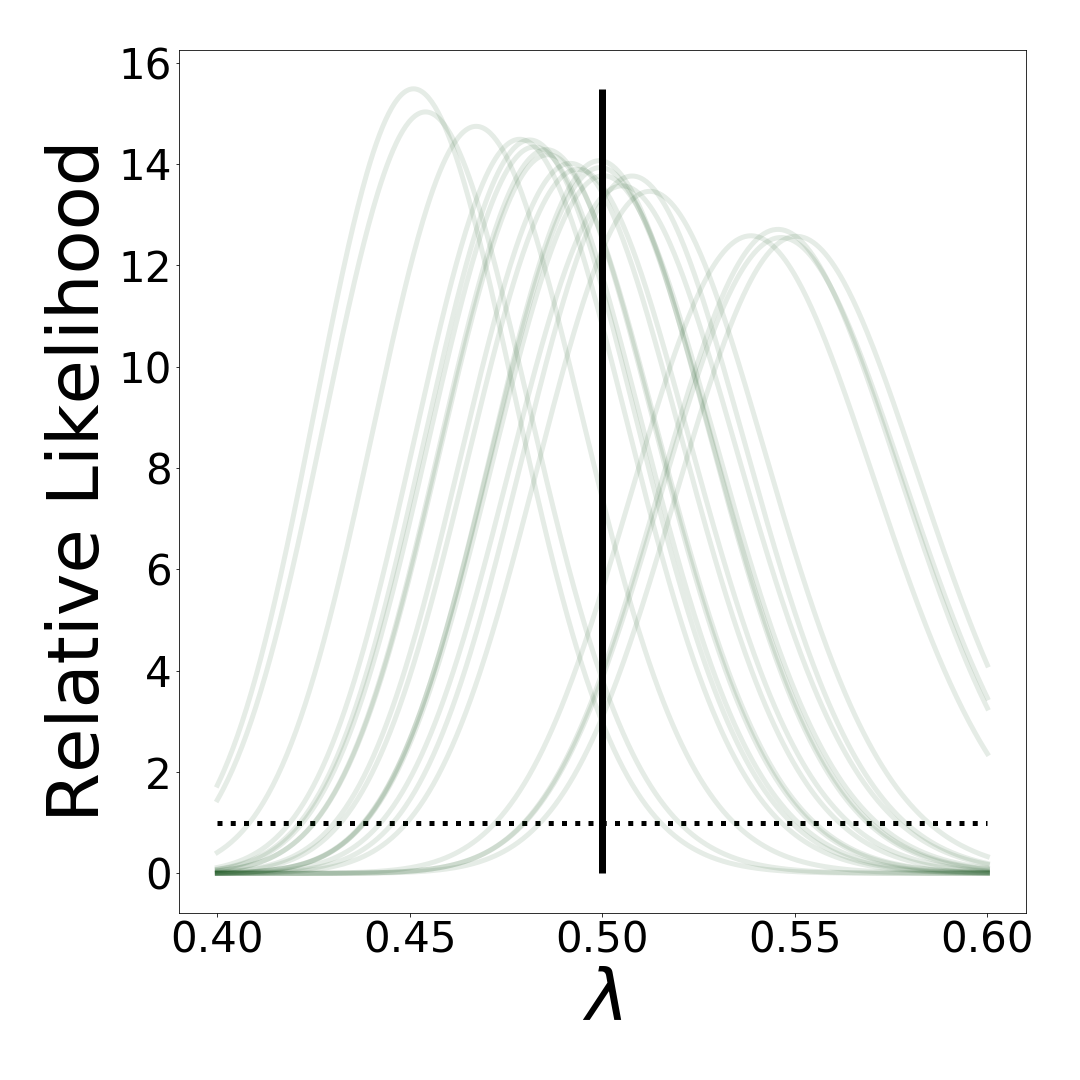
\includegraphics[width=13cm]{figures/posterior_stability_D10_sigma-10E-4}\\
        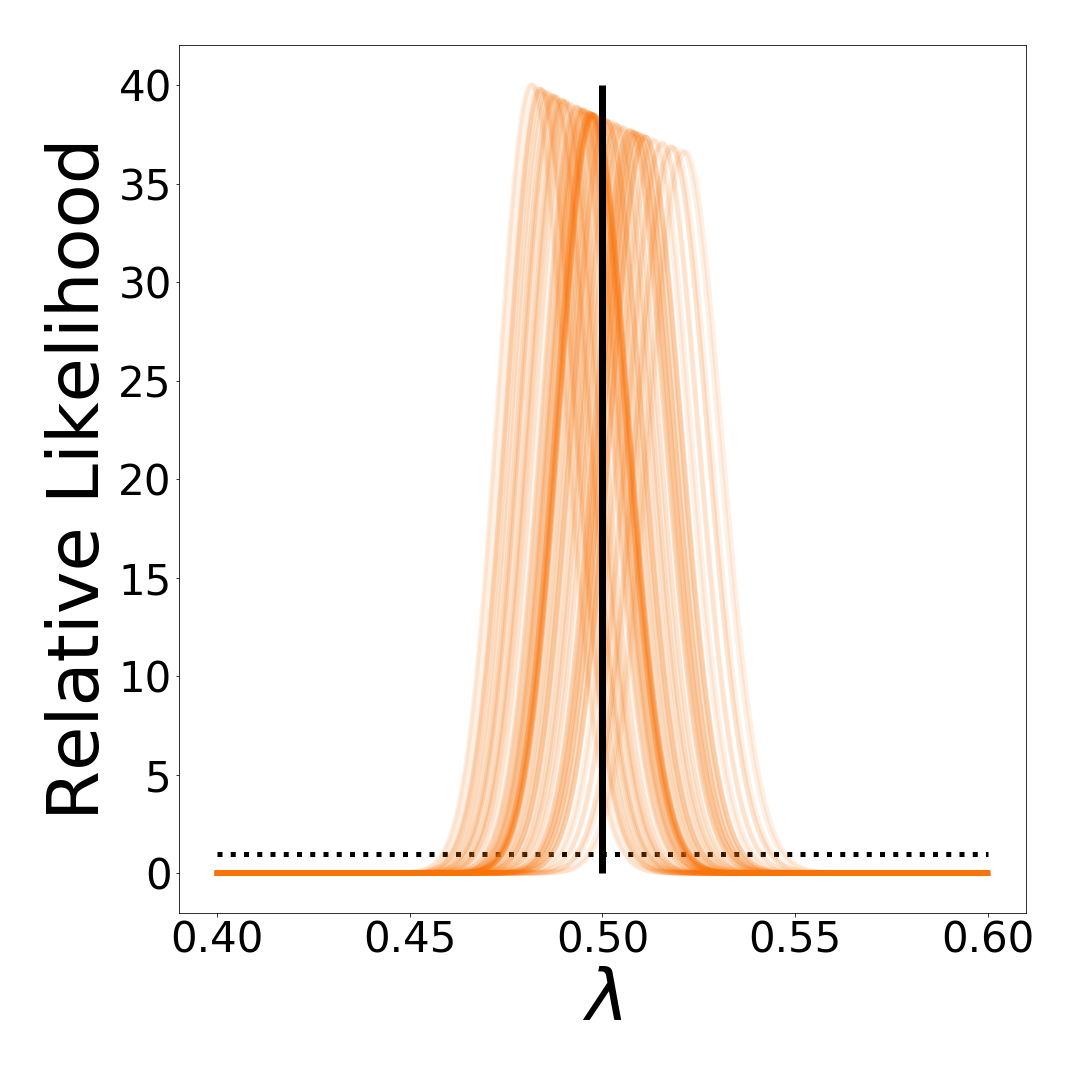
\includegraphics[width=13cm]{figures/updated_stability_D100_sigma-10E-4}
        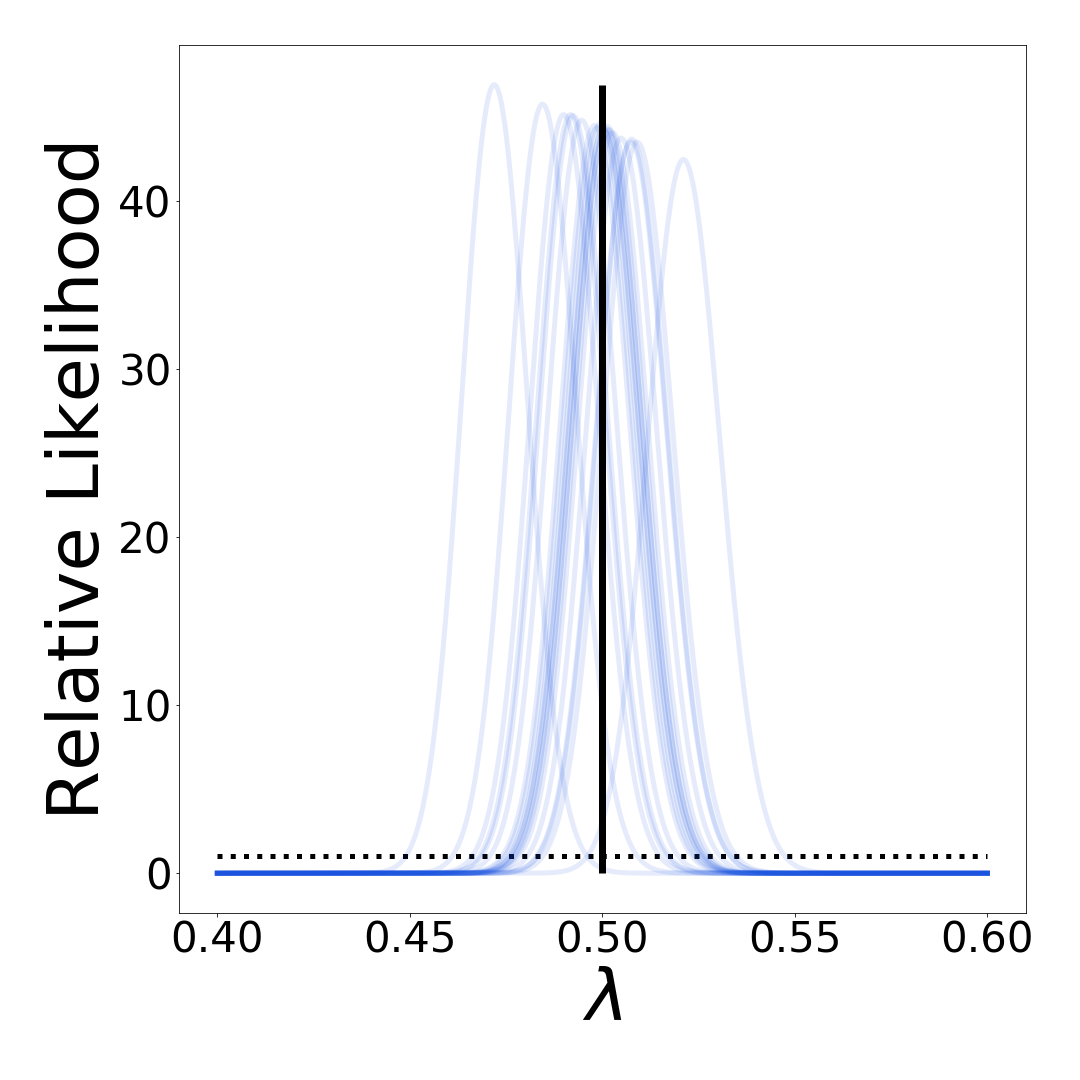
\includegraphics[width=13cm]{figures/posterior_stability_D100_sigma-10E-4}
        \vspace{-1cm}
        \caption{100 realizations of data for $D=10,100$ for Data Consistent Inversion (left) and Regular Bayes (right).}
    \end{figure}

\end{block}

  
\end{column}

\separatorcolumn
\end{columns}
\end{frame}

\end{document}
